\documentclass[a4paper,12pt]{article}
\usepackage{calc,amsmath,amssymb,amsfonts}
\usepackage[LGR,T1]{fontenc}
\usepackage[english, polish]{babel}
\usepackage[style=ieee,backend=bibtex]{biblatex}
\usepackage{graphicx}
\usepackage{subcaption}
\usepackage{geometry}
\usepackage{setspace}
\usepackage{comment}
\usepackage{algorithm}
\usepackage{algorithmic}
\usepackage{pdflscape}
\usepackage{pdfpages}
\usepackage{physics}
\usepackage{array}
\usepackage{booktabs}
\newtheorem{definition}{Definition}
\usepackage[hidelinks]{hyperref}
\usepackage{todonotes}


\addbibresource{bibliography.bib}

\author{Dawid Mazur}
\date{2024-09-16}

% \geometry{
%     left=3cm, right=2cm, top=2cm, bottom=2cm,
%     includehead, includefoot,
%     twoside
% }
% \setstretch{1.25}

\begin{document}

\selectlanguage{english}
\newpage
\tableofcontents

\newpage
\section{Introduction}\label{introduction}
Technological advancements in the XX century contributed to development of computer science, and the digital era has emerged. One of the modern advancements that we witness is the rapid growth of artificial intelligence, especially in the field of generative models, particularly introducing Generative Adversarial Networks in 2014 \cite{Goodfellow2014}, and Transformer architecture in  2017 \cite{Vaswani2023}. Certainly worth mentioning is the 2024 Nobel Prize in Physics for John J. Hopfield and Geoffrey E. Hinton. The motivation for the prize was as follows: ``for foundational discoveries and inventions that enable machine learning with artificial neural networks''. There are more generative-based models than those two mentioned, and this work will explore the application of other models.

The Restricted Boltzmann Machines (RBM), initially introduced in 1986 under the name Harmonium \cite{Smolensky1986}, fall into the generative models category due to their ability to learn a probabilistic distribution over its set of inputs. RBM is a widely used machine learning technique for unsupervised \cite{Decelle2023} and supervised tasks \cite{Dixit2021RBM_DWave}. We will use RBM as an unsupervised learning model in a pixel-level image segmentation context \cite{Wang2019, Agn2016}.

Segmentation is a core task in computer vision. It partitions an image into regions representing different objects or materials. Segmentation makes it possible to analyze image's structure accurately, and it has applications in many fields, such as medicine \cite{Wang2022} or satellite image analysis \cite{fajtl2020}.

In this work, we will focus on the segmentation of multispectral images. Multispectral images differ from ordinary images in that they capture information in multiple electromagnetic spectrum wavelengths \cite{Mengu2023}, not just the visible range. It allows for a deeper analysis of the properties of imaged objects, as each pixel contains spectral information in different bands \cite{Sifnaios2024}. Research on hyperspectral imaging at the pixel-level has grown in recent years, leading to an increasing number of scientific publications in this field \cite{Morchhale2016, González-Santiago2022, Yan2023, Sifnaios2024, Chen2024}.

Quantum computing is a multidisciplinary field that includes computer science, physics, and mathematics. Quantum computing leverages the principles of quantum mechanics to solve complex problems. One possible approach to using quantum computing, alongside the gate model \cite{Pereira2023}, is Adiabatic Quantum Computing (AQC) \cite{Kadowaki1998} and closely related quantum annealing. An interesting possibility is the use of quantum computing, both gate-based and AQC, in machine learning models \cite{schuld2021}. 

D-Wave Systems Inc. is a Canadian company that has pioneered the commercial application of quantum computing. This company has developed several generations of quantum processing units (QPU) based on various architectures known as Chimera, Pegasus, and Zephyr \cite{DWaveDocumentation}.

The goal of this work is to explore the possibility of using Restricted Boltzmann Machines for pixel-level analysis of multispectral images and segmentation of those images. We also aim to use the D-Wave's quantum annealer and compare the segmentation results with the classical RBM training method.

\section{Image Segmentation}\label{segmentation}
Image segmentation is an important area of research and application in the field of computer vision. It has wide applications in many fields, such as medicine \cite{Ma2024}, remote sensing \cite{Kemker2018}, and vision systems in autonomous vehicles \cite{Cakir2022}. It is the process of dividing an image into homogeneous regions. Formally, image segmentation can be defined as follows \cite{Pal1993}. If $F$ is the set of all pixels and $P: F \to \{\text{true},\text{false}\}$ is a homogeneity predicate defined on groups of connected pixels, then segmentation is a partitioning of the set $F$ into a set of connected subsets or regions $(S_{1},S_{2},\ldots,S_{n})$ such that \cite{Pal1993}:

\begin{equation}\label{segmentation_eq}
    \bigcup_{i=1}^{n} S_{i}=F \quad \text{with} \quad S_{i} \cap S_{j} = \emptyset, i \neq j.
\end{equation}

\noindent The homogeneity predicate $P(S_{i})=\text{true}$ for all regions $S_{i}$ and $P(S_{i} \cap S_{j})=\text{false}$, when $S_{i}$ is adjacent to $S_{j}$. Set $F$ is a digital image defined as \cite{Pal1993}:

\begin{equation}\label{digital_image}
    F_{W \times H}=[f(x,y)]_{W \times H},
\end{equation}

\noindent where $W$ and $H$ are image dimensions and $f(x,y) \in G_{L}=\{0,1, \ldots, L-1\}$ is a set of discrete levels of the feature value, $(x,y)$ denotes the spatial coordinate. Equation \eqref{digital_image} refers to monochrome images, although it could be extended to commonly used images in RGB or other color spaces by adding channel or band dimension. The extended form of Equation \eqref{digital_image} can be defined as:

\begin{equation}\label{digital_image_extended}
    F_{W \times H \times B}=[f(x,y,\lambda)]_{W \times H \times B},
\end{equation}

\noindent where $B$ is a band dimension. The Equation \eqref{digital_image_extended} represents the hyperspectral or multispectral image on which we intend to perform segmentation.

The task of image segmentation can be approached with a variety of algorithms, including both classical methods \cite{Chen2017} and those based on deep learning \cite{Badrinarayanan2017}. Among classical algorithms that are often used for segmentation are approaches like \cite{Chen2017}:

\begin{itemize}
    \item thresholding,
    \item region-based,
    \item edge-detection,
    \item clustering.
\end{itemize}

Clustering is an unsupervised machine learning class of algorithms that allows models to learn patterns in data without explicit labels. Segmentation with the classical clustering algorithm can be be implemented using \textit{e.g.}, $k$-means \cite{Dhanachandra2015} or Agglomerative Hierarchical Clustering \cite{Mohanta2002}. Both of these algorithms will be discussed in the following chapters, as they will be used to set a baseline for our model to exceed and to recognize the higher hierarchy of clusters returned by our model.

The following chapters will also discuss clustering using deep learning models, as the neural network architecture presented in this dissertation derives from deep learning.

\section{Unsupervised Learning}\label{unsupervised_learning}

Artificial intelligence is a technology at the intersection of mathematics and computer science. It includes a wide spectrum of methods and algorithms that enable machines to learn, resulting in a wide range of applications \cite{raschka2019, Goodfellow2016}. The origins of artificial intelligence are considered to be the Perceptron model presented conceptually in \cite{Mcculloch1943} and developed in \cite{Rosenblatt1958}. Literature \cite{raschka2019} proposes the following division of artificial intelligence algorithms:

\begin{itemize}
\item supervised learning,
\item unsupervised learning,
\item reinforcement learning.
\end{itemize}


Unsupervised learning is a fundamental approach in machine learning that allows models to learn patterns in data without explicit labels. The goal of learning in this context is to uncover the underlying structure of the dataset. The classic problems in which unsupervised learning is applied are clustering and dimensionality reduction. Clustering can be performed using a variety of algorithms \cite{Bindra2017}, including partitioning methods, density-based and hierarchical methods. Dimensionality reduction has traditionally been achieved using principal component analysis (PCA) \cite{Goodfellow2016}, but autoencoders have also proven to be highly effective for this task \cite{Wang2014}. 

In the context of this work, we will use several unsupervised learning algorithms, one to enable sufficient representation learning and dimensionality reduction and other clustering algorithms to perform image segmentation.

\subsection{Latent Bernoulli Autoencoder}\label{lbae_section}

Autoencoders are artificial neural networks used for unsupervised representation learning. Representation learning or feature learning is a process during which algorithms extract meaningful patterns from data to create representations usually in a lower dimension than the original data.

The autoencoder architecture is built from two separate networks. The first network, referred to as the encoder, executes the encoding operation $h = f(x)$, while the second one, known as the decoder, carries out the decoding operation $r = g(h)$. An autoencoder whose latent space  $h$ dimension is lower than the input data dimension is called undercomplete \cite{Goodfellow2016}. Learning an undercomplete representation forces the autoencoder to capture the most significant features of the training data.
When the encoder and decoder are linear and the loss function is the mean squared error, an undercomplete autoencoder learns to capture the same subspace as PCA. In this scenario, an autoencoder trained to reconstruct its input ends up learning the principal subspace of the training data as a byproduct. Autoencoders with nonlinear encoder transformation $f$ and nonlinear decoder transformation $g$ can therefore learn a more flexible and powerful nonlinear extension of PCA \cite{Goodfellow2016}. 

Autoencoder networks may be viewed as special cases of feed-forward networks and can be trained similarly, especially using gradient descent and back-propagation techniques. The learning process in an autoencoder involves minimizing a loss function, denoted by $L$, which quantifies the difference between the input and the reconstructed output \cite{Goodfellow2016}. A loss function is generally defined as:

\begin{equation}\label{loss}
    L(x,g(f(x))),
\end{equation}

\noindent where $L$ is a loss function penalizing  $g(f\left(x\right))$ for being dissimilar from  $x$. The loss function is typically defined as the mean squared error (MSE):

\begin{equation}\label{mse}
    \text{MSE} = \frac{1}{n} \sum_{i=1}^{n} (\mathbf{x}_i - \hat{\mathbf{x}}_i)^2,
\end{equation}

\noindent where $\mathbf{x}_i$ is an input data --- a vector of features and $\hat{\mathbf{x}}_i$ is the $\mathbf{x}_i$ reconstruction, which is obtained as an autoencoder output \cite{Goodfellow2016}.

Latent Bernoulli Autoencoder (LBAE) belongs to the generative models' category, and its idea is based on a class of autoencoders called Variational Autoencoders (VAE) \cite{fajtl2020}. The interesting LBAE property is that the hidden layer is binarized by \cite{fajtl2020}:

\begin{equation}\label{lbae_latent_space}
    h_{i} = 
    \begin{cases}
        1, & \text{if } \tanh(\mathbf{z}_i) \geq 0 \\
        -1, & \text{if } \tanh(\mathbf{z}_i) < 0
    \end{cases},
\end{equation}

\noindent where $\mathbf{z}_i$ is the input data transformed by the encoder. The importance of this property will be highlighted in the methodology section of this work.

\subsection{Restricted Boltzmann Machines}\label{rbm_section}
In contrast to traditional approaches in machine learning and deep learning, structured probabilistic models offer a different paradigm. These models focus on representing probability distributions through graph-based structures, defined as:

\begin{equation}
    G=(V,E),
\end{equation}

\noindent where $V$ represents vertices and $E$ represents edges in a given graph $G$. Each vertex represents a random variable, and each edge represents direct interaction between random variables \cite{Goodfellow2016}. The type of connection between vertices defines whether the model is directed or undirected.

Restricted Boltzmann Machines are undirected graphical, energy-based models that contain a layer of observable variables and a layer of latent variables. Referring to the layer of observable variables, we will speak of the visible layer marked as $\mathbf{v}$, and referring to the layer of latent variables, we will speak of the hidden layer marked as $\mathbf{h}$ \cite{Goodfellow2016}\cite{Tieleman2008}.

\begin{figure}[h]
    \centering
    {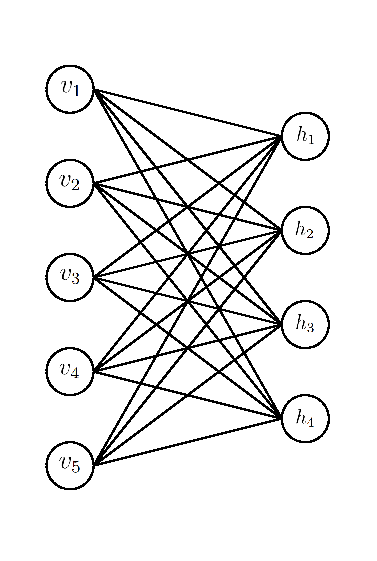
\includegraphics[width=0.35\textwidth]{figures/unsupervised_learning/rbm.pdf}}
    \caption[The general architecture of the RBM graph.]{The general architecture of the RBM graph. Here, $v_i \in \{1, 2, \ldots, 5\}$ denote vertices --- neurons in visible layer $\mathbf{v}$ and $h_i \in \{1, 2, 3, 4\}$ denote neurons in hidden layer $\mathbf{h}$. Each vertex connects through edges to all vertices in the other set but to none in its own set.}
    \label{fig:general_rbm}
\end{figure}

Based on \cite{Goodfellow2016, Dixit2021RBM_DWave}, we can define the joint probability distribution of the RBM as follows:

\begin{equation}\label{rbm_joint_prob_dist_x}
    P(\mathbf{x}) = \frac{1}{Z} e^{-E(\mathbf{x})},
\end{equation}

\noindent where $\mathbf{x} \in \{0,1\}^n$. Equation \eqref{rbm_joint_prob_dist_x} can be also written with respect to $\mathbf{v}$ and $\mathbf{h}$ layers as \cite{Goodfellow2016}:

\begin{equation}\label{rbm_joint_prob_dist}
    P(\mathbf{v}, \mathbf{h}) = \frac{1}{Z} e^{-E(\mathbf{v}, \mathbf{h})},
\end{equation}

\noindent where $\mathbf{v} \in \{0,1\}^n$ and $\mathbf{h} \in \{0,1\}^n$. The energy function for the RBM is given by:

\begin{equation}\label{rbm_energy_function}
    E(\mathbf{v},\mathbf{h})=-\mathbf{b}^T\mathbf{v}-\mathbf{c}^T\mathbf{h}-\mathbf{v}^T\mathit{\mathbf{W}\mathbf{h}},
\end{equation}

\noindent where $\mathbf{b},\mathbf{c} \in \mathbb{R}^n$ are biases and  $\mathbf{W} \in \mathbb{R}^{n \times n}$ is a connection matrix. The following equation gives the partition function:

\begin{equation}\label{rbm_partition_function}
    Z = \sum_{\mathbf{v},\mathbf{h}} e^{-E(\mathbf{v},\mathbf{h})}.
\end{equation}

\noindent The partition function is intractable to compute and the joint probability distribution being a function of $Z$ is also computationally intractable. However, due to RBM's graph structure, the conditional distributions $P(\mathbf{h}|\mathbf{v})$ and $P(\mathbf{v}|\mathbf{h})$ are simple to compute. $P(\mathbf{h}|\mathbf{v})$ is given by:

\begin{equation}\label{p_h_cond_v}
    P(\mathbf{h} \mid \mathbf{v}) =\frac{P(\mathbf{v},\mathbf{h})}{P(\mathbf{v})},
\end{equation}

\noindent where $P(\mathbf{v})$ is given by:

\begin{equation}\label{p_v}
    P(\mathbf{v}) = \frac{\sum_\mathbf{h} e^{-E(\mathbf{v},\mathbf{h})}}{Z}.
\end{equation}

\noindent By substituting values from equations \eqref{rbm_joint_prob_dist}, \eqref{partition_function}, \eqref{p_v} into \eqref{p_h_cond_v} we receive:

\begin{equation}
    P(\mathbf{h} \mid \mathbf{v}) = \frac{e^{\sum_j c_j h_j + \sum_j (\mathbf{v}^T \mathbf{W})_j \mathbf{h}_j}}{Z'},
\end{equation}

\noindent where $Z'$ is:

\begin{equation}
    Z' = \sum_\mathbf{h} e^{\mathbf{c}^T \mathbf{h} + \mathbf{h}^T \mathbf{W}\mathbf{v}},
\end{equation}

\noindent and therefore,

\begin{equation}
    P(\mathbf{h} \mid \mathbf{v}) = \frac{1}{Z'} \prod_j e^{\sum_j c_j h_j + (\mathbf{v}^T \mathbf{W})_j \mathbf{h}_j}.
\end{equation}

\noindent We can denote this as:

\begin{equation}
    \tilde{P}(\mathbf{h} \mid \mathbf{v}) = e^{c_j h_j + (\mathbf{v}^T \mathbf{W})_j \mathbf{h}_j}.
\end{equation}

\noindent It is now a simple matter of normalizing the distributions over the individual binary $h_j$:

\begin{equation}
    P(h_j=1 \mid \mathbf{v}) = \frac{\tilde{P}(h_j=1 \mid \mathbf{v})}{\tilde{P}(h_j=0 \mid \mathbf{v}) + \tilde{P}(h_j=1 \mid \mathbf{v})},
\end{equation}

\begin{equation}
    P(h_j=1 \mid \mathbf{v}) = \frac{e^{c_j + (\mathbf{v}^T\mathbf{W})_j}}{e^{0} + e^{c_j + (\mathbf{v}^T\mathbf{W})_j}},
\end{equation}

\begin{equation}\label{p_hj_1_mid_v_show_sigmoid}
    P(h_j=1 \mid \mathbf{v}) = \frac{1}{1 + e^{-\mathbf{c}_j - (\mathbf{v}^T\mathbf{W})_j}}.
\end{equation}

\noindent Using the formula for the sigmoid function:

\begin{equation}\label{sigmoid}
    \sigma(x) = \frac{1}{1 + e^{-x}},
\end{equation}

\noindent we can denote Equation \eqref{p_hj_1_mid_v_show_sigmoid} as:

\begin{equation}\label{p_hj_1_mid_v}
    P(h_j = 1 \mid \mathbf{v}) = \sigma (c_j + (\mathbf{v}^T\mathbf{W})_j).
\end{equation}

\noindent Similarly we can obtain $P(v_j = 1 \mid \mathbf{h})$ by:

\begin{equation}\label{p_vi_1_mid_h}
    P(v_i = 1 \mid \mathbf{h}) = \sigma (b_i + (\mathbf{h}^T\mathbf{W})_i).
\end{equation}

RBM training is based on maximizing the log-likelihood of the training data. The log-likelihood is given by \cite{Dixit2021RBM_DWave}:

\begin{equation}\label{log_likelihood}
    l(\theta) = \sum_{t=1}^N \log P(\mathbf{v}^{(t)}),
\end{equation}

\noindent and this equation can be denoted as \cite{Dixit2021RBM_DWave}:

\begin{equation}\label{log_likelihood_denoted}
    l(\theta) = \sum_{t=1}^N \log \sum_{\mathbf{h}} e^{-E(\mathbf{v}^{(t)}, \mathbf{h})} - N \cdot \log \sum_{\mathbf{v}, \mathbf{h}} e^{-E(\mathbf{v}, \mathbf{h})},
\end{equation}

\noindent where $\theta=\{\mathbf{W}, \mathbf{b}, \mathbf{c}\}$ and $\mathbf{v}^{(t)}$ is a sample from the training dataset with N records. The gradient of the log-likelihood is given by \cite{Dixit2021RBM_DWave}:

\begin{equation}
    \nabla_{\theta} l(\theta) = \sum_{t=1}^N \frac{\sum_\mathbf{h} e^{-E(\mathbf{v}^{(t)}, \mathbf{h})} \nabla_{\theta} \left(-E(\mathbf{v}^{(t)}, \mathbf{h})\right)}{\sum_{\mathbf{v}, \mathbf{h}} e^{-E(\mathbf{v}, \mathbf{h})}} - N \cdot \frac{\sum_{\mathbf{v}, \mathbf{h}} e^{-E(\mathbf{v}, \mathbf{h})} \nabla_{\theta} \left(-E(\mathbf{v}, \mathbf{h})\right)}{\sum_{\mathbf{v}, \mathbf{h}} e^{-E(\mathbf{v}, \mathbf{h})}},
\end{equation}

\begin{equation}
    \nabla_{\theta} l(\theta) = \sum_{t=1}^N \langle \nabla_{\theta} \left(-E(\mathbf{v}^{(t)}, \mathbf{h})\right) \rangle_{P(\mathbf{h} | \mathbf{v}^{(t)})} - N \cdot \langle \nabla_{\theta} \left(-E(\mathbf{v}, \mathbf{h})\right) \rangle_{P(\mathbf{v}, \mathbf{h})},
\end{equation}

\noindent  where $\langle \cdot \rangle_{P(\mathbf{v},\mathbf{h})}$ is the expectation value with respect to the distribution $P(\mathbf{v}, \mathbf{h})$. This is a decomposition into positive phase and negative phase. The RBM is an example of a model for which positive-phase and negative-phase are, respectively, easy and difficult \cite{Dixit2021RBM_DWave, Goodfellow2016}.

Negative-phase $\nabla_{\theta} (-E(\mathbf{v}, \mathbf{h}))$ is hard to compute but its approximation can be obtained using the Monte Carlo Markov Chain methods (MCMC) \cite{Goodfellow2016}. One of the MCMC algorithms family is the contrastive divergence (CD) algorithm. CD uses the dependencies described in the Equations \eqref{p_hj_1_mid_v} and \eqref{p_vi_1_mid_h}. Alternatively, the negative-phase can be calculated using samples drawn from a quantum annealer \cite{Dixit2021RBM_DWave}. The use of annealing can lead to more efficient sampling than MCMC algorithms, which can struggle to correctly approximate the negative phase of the gradient \cite{Goodfellow2016}. While CD relies on limited Gibbs sampling steps and can get stuck in local minima, annealing explores more global configurations, improving sampling accuracy and learning dynamics in challenging scenarios.

\subsection{Cluster Analysis}\label{cluster_analysis_section}

Cluster analysis is a category of unsupervised learning algorithms that seek to divide a given set of objects into homogeneous clusters \cite{Bratchell1989}. In the context of image segmentation, cluster analysis divides an image into regions with similar properties.

Clustering algorithms are divided into \cite{Bindra2017}:

\begin{itemize}
    \item partitional clustering,
    \item hierarchical clustering,
    \item density-based clustering.
\end{itemize}

\noindent Each of these approaches offers unique advantages in dealing with different underlying data structure. Partitional clustering methods, attempt to directly partition a dataset into k distinct clusters. Hierarchical clustering methods construct a hierarchy of clusters by successively merging smaller clusters (agglomerative approach) or splitting larger clusters (divisive approach). Density-based methods define clusters based on high-density regions, effectively identifying clusters of arbitrary shapes and distinguishing noise or outliers \cite{Bindra2017}.

The following chapters of this work will be devoted to an algorithm based on partial clustering, which is $k$-means, and a hierarchical clustering algorithm, which is Agglomerative Hierarchical Clustering (AHC).

\section{Quantum Computing}\label{quantum_computing}

Quantum computing is a domain that has gained immense interest in recent years in both the scientific and industrial sectors \cite{Flother2023, Ahmed2024, Orus2019, Phillipson2024}. Taking advantage of the unique properties of quantum mechanics, such as superposition and entanglement, quantum computers promise a breakthrough in information processing, offering computational capabilities unavailable to classical computers.

Traditional computers operate on bits, which can take the value of 0 or 1. In contrast, quantum computers operate on qubits (quantum bits), which, due to the phenomenon of superposition can exist in a state that is a linear combination of states ``0'' and ``1'', enabling quantum computers to process information in different ways compared to classical computers. In addition, quantum entanglement allows the states of qubits to be non-locally connected, leading to performing some computational tasks exponentially faster than classical algorithms \cite{Datta2005}.

A quantum system evolves according to the Schr\"odinger equation \cite{schuld2021}:

\begin{equation}\label{shrodinger}
    i \hbar \frac{d}{dt} \ket{\psi(t)} = H(t) \ket{\psi(t)},
\end{equation}

\noindent where $\ket{\psi}$ is the quantum state of the system at the time $t$ and $H(t)$ is the time-dependent Hamiltonian of a given system. $\hbar$ is Planck’s constant. Hamiltonian operator corresponds to the total energy of the system. The possible energies the system can have are the eigenvalues of the $H$ operator \cite{schuld2021, McMahon2008}.

\subsection{Ising Model and Quadratic Unconstrained Binary Optimization}\label{inig_qubo_section}

Ising model classically refers to disordered magnetic alloys containing strongly interacting ions immersed in a weakly interacting substrate [7]. We can interpret such an arrangement as randomly interacting spins up $(\uparrow)$ or down $(\downarrow)$ placed on lattice nodes. We can denote such an arrangement by an undirected graph $G=(V,E)$ \cite{Jałowiecki2023}. For each vertex, we assign a spin variable $s_i$ and a local magnetic field  $h_i$. To each edge, we assign an interaction strength $J_{ij}$. For such a system we can define a Hamiltonian:

\begin{equation}\label{isingH}
    H_{\mathrm{ising}}\left(s\right)=-\sum _{\left\langle i\right.,\left.j\right\rangle }J_{ij}s_is_j-\sum _ih_is_i,
\end{equation}

\noindent where $s_i{\in}\{-1,1\}$, $J_{ij}{\in}\mathbb{R}$, $h_i{\in}\mathbb{R}$. An Ising model with fixed coefficients is used to find the given system's ground state, it's lower energy state of a system's Hamiltonian. However, the Ising model is not the only tool to find the given system's ground state; the other one is Quadratic Unconstrained Binary Optimization (QUBO).

\begin{figure}
    \centering
    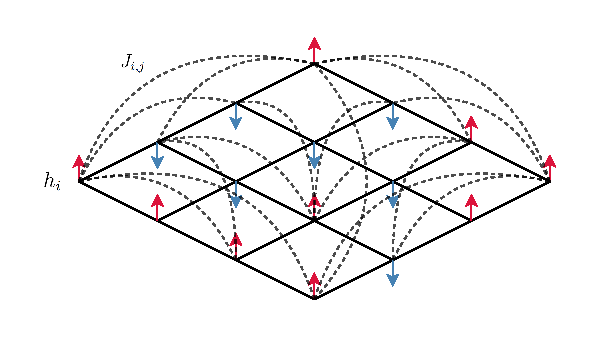
\includegraphics[width=0.8\linewidth]{figures/quantum_computing/ising_spinglass.pdf}
    \caption[Symbolic representation of Ising model.]{Symbolic representation of Ising model defined on the graph with $N=16$ vertices. $J_{i,j}$ denotes coupling strength associated with an edge between $i$-th and $j$-th node, and $h_i$ denotes qubit bias associated with $i$-th node.}
    \label{fig:symbolic_ising}
\end{figure}

What distinguishes QUBO from the Ising model is that QUBO uses binary variables $q_i{\in}\mathbb{B}=\{0,1\}$, instead of $s_i{\in}\{-1,1\}$ spin variables. QUBO problem can be defined as minimizing the objective function:

\begin{equation}
    \min_{q{\in}\{0,1\}^n}f_Q(q).
\end{equation}

\noindent The objective function $f_Q: \mathbb{B}^n \to \mathbb{R}$ is in the form given by:

\begin{equation}
    f_Q(x)=q^{T}Qq,
\end{equation}

\noindent where $Q \in \mathbb{R}^{n \times n}$ is upper triangular matrix, whose entries $Q_{ij}$ define a weight for each pair of indices $i,j \in \{1, 2, \ldots, n\}$. The objective function can be transformed to the following form:

\begin{equation}
    f_Q(q)=\sum _iQ_{ii}q_i+\sum _{i<j}Q_{ij}q_iq_j,
\end{equation}

\noindent which makes the QUBO problem and the Ising model essentially equivalent. To express the Ising model as a QUBO problem, we introduce the substitution $s_i=2q_i-1$ and we assign $a_i$ and $b_{ij}$ symbols to denote respectively linear and quadratic QUBO coefficients. Values for $a_i$ and $b_{ij}$ are as follows \cite{Jałowiecki2023}:

\begin{equation}\label{a_and_b_qubo}
    a_i = 4J_{ij}, \quad b_{ij} = 2h_i - 2\sum_{\left\langle i\right.,\left.j\right\rangle}J_{ij},
\end{equation}

\noindent what results in the following form of $f_Q$:

\begin{equation}
f_Q(q)=\sum _ia_iq_i+\sum _{i<j}b_{ij}q_iq_j,
\end{equation}

\noindent which differs from \eqref{isingH} by a constant value, although it is irrelevant to the optimization process \cite{Jałowiecki2023}.

\subsection{Adiabatic Quantum Computation and Quantum Annealing}\label{aqc_qa_section}

The core concept of Adiabatic Quantum Computing (AQC) relies on the adiabatic theorem \cite{Farhi2000}, which states that if a quantum system begins in the ground state of its initial Hamiltonian and the Hamiltonian changes slowly enough, the system will remain in its ground state throughout the evolution. 

The time-dependent Hamiltonian $H(t)$ is constructed from  $H_{\mathrm{init}}$ and $H_{\mathrm{target}}$. The adiabatic evolution of a state transforms the known ground state of the $H_{\mathrm{init}}$ into the unknown ground state of the $H_{\mathrm{target}}$. $H(s)$ is given by \cite{Kumar2018, Głomb2023}:

\begin{equation}\label{H(s)}
    H(s) = (1 - s) H_{\mathrm{init}} + s H_{\mathrm{target}},
\end{equation}

\noindent where $s=\frac{t}{T} \in [0, 1]$ and $T$ is the total evolution time, and it controls the rate at which $H(s)$ or $H(t)$ is varying. In AQC, the slower the evolution process, the better the approximate solution is obtained \cite{Calude2015}; this is why, in practice, the annealing approach is being used.

Annealing is a process in metallurgy that involves slowly cooling metal to achieve a state with the lowest possible internal energy, resulting in greater strength and structural stability \cite{Ferrer2001}. In this process, the metal atoms move freely at high temperatures, and the slow reduction of temperature allows them to gradually arrange themselves in a stable configuration.

Simulated annealing (SA) is an optimization algorithm inspired by this physical process. SA treats the optimization problem as a physical system, with energy representing the objective function value and temperature controlling the probability of accepting inferior solutions. The algorithm starts at a high temperature, where energy-increasing movements are allowed, and then the temperature slowly decreases to find the global minimum of the objective function \cite{Benedetti2021}.

Quantum annealing (QA) is an extension of the idea of simulated annealing that uses quantum effects to search the solution space. Unlike SA, which relies on classical temperature perturbations, QA uses quantum fluctuations to overcome energy barriers. Optimization problems, solvable by QA, are most often represented in terms of an Ising model. Although Quantum Annealing, in principle, follows similar scheme as Adiabatic Quantum Computing, the difference is that system evolution in QA is not necessarily adiabatic \cite{Vinci2017}.

Quantum annealing has the potential to be used for data clustering by transforming the optimization problem of the clustering cost function into the form of a quadratic binary optimization problem. QA makes it possible to search the solution space more efficiently and deal better with local minima compared to classical methods such as k-means \cite{Kumar2018}.

\subsection{D–Wave's Quantum Processing Units}\label{dwave_qpu_section}

D-Wave uses various architectures in its processors. The basic topology is Chimera and its architecture is designed to provide flexibility in mapping optimization problems onto a physical quantum system \cite{schuld2021}. However, the graph structure, like that of Chimera, introduces some limitations, \textit{e.g.}, not all qubits are directly connected to each other. 

Qubits in the Chimera topology are placed on a square grid of unit cells. Each cell includes two groups of four qubits and each qubit is connected to four qubits from the opposite group forming $K_{4,4}$ complete bipartite graph, illustrated in the Figure \ref{fig:unitcell}. 

\noindent Such cells are then combined into a two-dimensional grid, allowing the system to scale to a larger number of qubits and enable more complex interactions. Chimera layout is denoted by $C_n$, where $n$ is the width and the height of the grid and in such configuration, each qubit is connected to a maximum of 6 qubits, the total number of qubits is $8n^2$ and the total number of couplers is $16n^2 + 8(n - 1)^n$ \cite{Jałowiecki2023}. The couplers connecting qubits in the same unit cell are called internal and the couplers connecting qubits belonging to different cells are called external. An example of Chimera topology is shown in the Figure~\ref{fig:chimera_graph}.

The Pegasus $P_3$ architecture, illustrated in Figure \ref{fig:pegasus_graph}, represents the next generation of the Chimera topology. This topology introduces some upgrades to qubit connectivity. Firstly, the internal couplers not only connect qubits within the same unit cell but also link qubits in adjacent unit cells. Secondly, a new type of connection, referred to as odd couplers, is introduced within the unit cells. Each Pegasus unit cell consists of 24 qubits organized into three Chimera unit cells. The Pegasus topology, denoted by $P_n$, features $n$ rows and $n$ columns of unit cells and contains a total of $24n(n - 1)$ qubits \cite{Jałowiecki2023}.

D–Wave's QPU uses Ising Hamiltonian from Equation \eqref{isingH} in a transformed form~\cite{DWaveDocumentation}:

\begin{equation}\label{dwaveH}
    H_{\mathrm{ising}}\left(s\right)=\frac{-A\left(s\right)} 2\left(\sum _i\widehat {\sigma
}_x^{\left(i\right)}\right)+\frac{B(s)} 2\left(\sum _ih_i\widehat {\sigma }_z^{\left(i\right)}+\sum
_{i>j}J_{i,j}\widehat {\sigma }_z^{\left(i\right)}\widehat {\sigma }_z^{\left(j\right)}\right),
\end{equation}

\noindent where $\widehat {\sigma }_x^{\left(i\right)}$, $\widehat {\sigma }_z^{\left(i\right)}$, $\widehat {\sigma
}_z^{\left(j\right)}$ are Pauli matrices on qubit $q_i$, $h_i$ and $J_{i,j}$ are respectively the qubit biases and coupling strengths, $s = \frac{t}{T}$, where $t$ is time, and $T$ is the total time of the anneal. The relative energy of each state depends on the biases of qubits and couplers between them. The $A(s)$ is the tunneling energy, and the $B(s)$ is the problem Hamiltonian energy at $s$. Both are expressed as energies in units of Joules, as is standard for a Hamiltonian. A linear anneal sets $s = \frac{t}{T}$, where $t$ is time, and $T$ is the total time of the anneal. At $t = 0$, $A(0) > B(0)$, which leads to the quantum ground state of the system where each spin is in a delocalized combination of its classical states. As the system is annealed, $A$ decreases and $B$ increases until $T$ when the final state of the qubits represents a low-energy solution to a problem Hamiltonian.

Hamiltonian from Equation \eqref{dwaveH} is composed of two parts: 
$H_{\mathrm{init}}$ and $H_{\mathrm{final}}$:

\begin{equation}\label{DWaveHinit}
    H_{\mathrm{init}}=\frac{-A\left(s\right)} 2\left(\sum _i\widehat {\sigma }_x^{\left(i\right)}\right),
\end{equation}

\begin{equation}\label{DWaveHfinal}
    H_{\mathrm{final}}=\frac{B(s)} 2\left(\sum _ih_i\widehat {\sigma }_z^{\left(i\right)}+\sum _{i>j}J_{i,j}\widehat
{\sigma }_z^{\left(i\right)}\widehat {\sigma }_z^{\left(j\right)}\right).
\end{equation}

\noindent  $A(s)$ represents the tunneling energy, and $B(s)$ refers to the Hamiltonian energy of the problem in a given time step $s$.

\section{Methodology}\label{methodology}
This chapter will present a detailed concept of a neural network model designed for the segmentation of multispectral images. In what follows, we discuss image data preprocessing, implementation details of the model's components, their integration, and methods of their evaluation, especially in the context of multispectral image segmentation.

\subsection{Data Preprocessing}\label{data_preprocessing_section}
The preparation of spectral data for processing by the neural network model proposed later in this work included transformations that are standard in the field of machine learning.

The documentation of the dataset \cite{Romaszewski2021} describes some of the hyperspectral channels as “noisy”, and we decided that the indicated spectral bands should be removed from further processing. We also decided to remove from hyperspectral images pixels whose position $(x,y)$ corresponded to the label ``0'' (which is the background) in the ground truth image; by such action, we wanted to achieve better clustering results because the background in the studied dataset is not homogeneous --- the neural network model would try to assign background pixels to different classes.

The following data transformations were to perform normalization, shuffle the data, and divide the data into training, validation, and test sets. Scaling to the interval $\langle 0, 1 \rangle$ was chosen as a standard normalization method in machine learning \cite{raschka2019} but was also used for processing hyperspectral images \cite{Głomb2023}. Data shuffling was used to reduce the influence of sequential pixel order. Data partitioning was done according to the Pareto principle: first, the data were divided into a training set and a test set in a ratio of $0.8:0.2$, and then the training set was further split into a training and validation set, also in a ratio of $0.8:0.2$.

\subsection{Proposed Model}\label{proposed_model_section}
Our proposed model, shown in Figure \ref{fig:proposed_model_pipeline}, accepts preprocessed input data as described above section of this work. Our proposed model consists of two main parts. The part, that this work aim to study is the Restricted Boltzmann Machines (RBM) part, and the second one is the Latent Bernoulli Autoencoder (LBAE) part. RBM requires binary data as input, so the data must be encoded into binary form. In our model, LBAE's encoder will be used for this task as it is proven to work well in similar task \cite{QBM4EO}. The data flow starts with LBAE, so we will start describing our proposed model with it.

\begin{figure}[h]
    \centering

    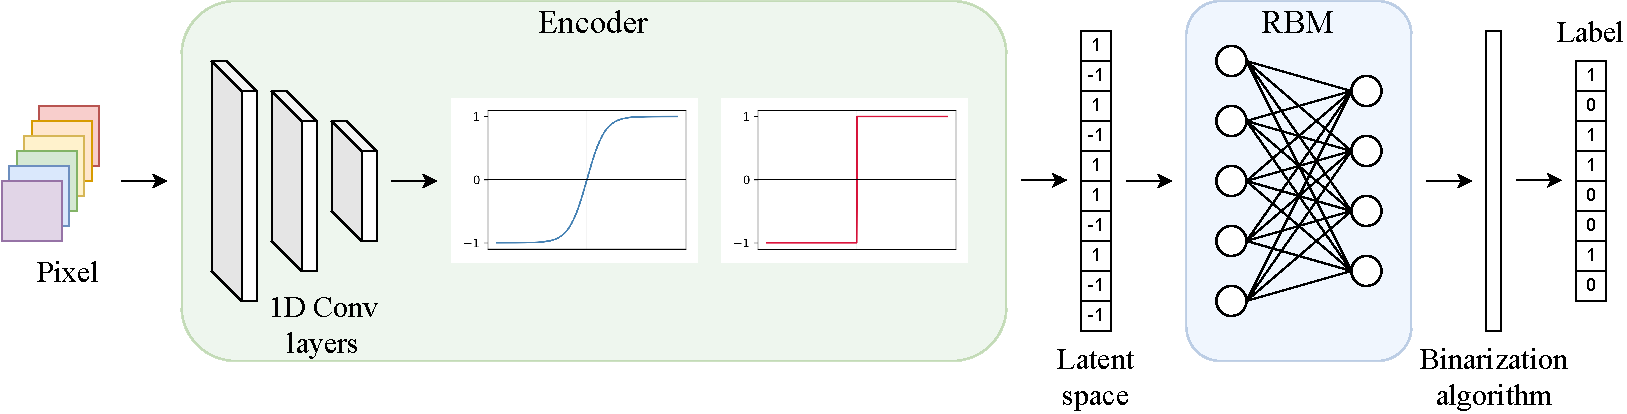
\includegraphics[width=1\textwidth]{figures/metodology/pipeline.pdf}
    \caption[Proposed model pipeline.]{Proposed model pipeline. The pipeline processes spectral pixel data through the LBAE encoder, which consists of one-dimensional convolutional layers followed by a $tanh$ activation and binarization (as described in Equation \eqref{lbae_latent_space}). The resulting binary representation is forwarded into the visible layer of the RBM, where the neuron's activation probabilities in a hidden layer are binarized, and the resulting binary vector is considered as a label.}
    \label{fig:proposed_model_pipeline}
\end{figure}

\subsubsection{Data Processing Module --- LBAE}\label{lbae_implementation}
LBAE is an autoencoder which was introduced in \cite{fajtl2020} and implemented in \cite{QBM4EO}. It contains convolutional layers in both encoding and decoding parts. Our approach relies on the work done in the \cite{QBM4EO}. However, our approach explores the possibility of pixel-level analysis in the context of hyperspectral images, so we had to adjust \cite{QBM4EO} implementation of the LBAE. This adjustment consisted of changing the convolution layers from two to one-dimensional. The rest of the network and its layers will stay the same as in \cite{QBM4EO} as this project obtained satisfactory performance. LBAE will be trained using techniques such as back-propagation and gradient descent as described in Section \ref{lbae_section}. Our LBAE transforms the spectral (already preprocessed) data into a binary representation. Input data is a 112-element vector, which will be transformed through convolutional layers. Due to the undercomplete architecture of this autoencoder, the dimension of this vector shrinks accordingly to each convolution layer as it is described by a given formula \cite{PyTorchDocumentation}:

\begin{equation}
    L_{\text{out}} = \left\lfloor \frac{L_{\text{in}} + 2 \times \text{padding} - \text{dilation} \times (\text{kernel size} - 1) - 1}{\text{stride}} + 1 \right\rfloor,
\end{equation}

\noindent where $L_{\text{out}}$ is the output length of the vector applying the convolutional layer, and $L_{\text{in}}$ is the input vector length. The term $\text{padding}$ refers to the number of elements added to each input side to control the output length. The $\text{dilation}$ factor specifies the spacing between elements in the convolution kernel, effectively increasing the kernel's receptive field, $\text{kernel\_size}$ represents the size of the convolutional kernel, or the number of samples covered by the kernel in one pass, while $\text{stride}$ denotes the number of steps the kernel moves with each application. 

\begin{table}[ht]
    \centering
    \caption{Parameters of the convolutional layers in the LBAE encoder.}
    \begin{tabular}{@{}lcccc@{}}
    \toprule
    Layer & Padding & Dilation & Kernel Size & Stride \\ \midrule
    Conv1 & 1       & 1        & 3           & 1      \\
    Conv2 & 1       & 1        & 4           & 2      \\
    Conv3 & 1       & 1        & 4           & 2      \\
    Conv4 & 1       & 1        & 3           & 1      \\ \bottomrule
    \end{tabular}
    \label{tab:conv_params}
\end{table}

The vector that we aim to obtain, which is a vector in the latent space of our autoencoder, has 28 binary elements. We postulate that if the values of both metrics, which we will observe, the Euclidean distance and the spectral angle distance computed between the input spectral vector and reconstructed spectral vector, are low, the hidden representation in the latent space is good. This binary representation will serve as an input to the RBM. 

\subsubsection{Data Clustering Module --- RBM}\label{rbm_implementation}
RBM is a neural network that accepts binary data as its input, and by the LBAE encoding part, we can obtain a binary representation of the original data. The number of neurons in the visible layer of our RBM is determined by input data dimension and LBAE encoder convolutional layers; in the case of our experiments, that would be 28 neurons. 

We will conduct experiments to train the RBM model with a fixed number of neurons in its visible layer and a changing number of neurons in its hidden layer $h_i \in \{3, 4, \ldots, 28\}$ using CD-$1$ algorithm. Our approach is to take RBM's hidden layer neurons activation probabilities calculated with Equation \eqref{p_hj_1_mid_v} and binarize those probabilities, and then the obtained binary vector is a label. The binarization threshold will be selected as follows: for each $th_i \in \{0.1, 0.2, \ldots, 0.9\}$, we will compute adjusted rand score (ARS) between true labels and predicted labels. Then we will check for which threshold we obtained the highest ARS, and for this threshold, we compute other metrics. Then, while having trained RBM models, we proceed to determine the best one by comparing them via V-measure, a meta metric whose value depends on homogeneity, completeness, and an additional $\beta$ parameter. Authors of \cite{Rosenberg2007} do not suggest how to choose $\beta$ value, however it is said by them that $\beta \in [0,1]$ promotes homogeneity. We will conduct an experiment that explores, for which model we obtained, the highest value of V-measure for $\beta_i \in \{0, 0.01, \ldots, 1\}$. The RBM architecture that most frequently obtains the highest V-measure scores will be selected as the best one, and we will proceed to experiments with simulated annealing (SA) and quantum annealing (QA) on this architecture.

The utilization of annealing to train Restricted Boltzmann Machines represents a novel approach to optimizing model parameters by exploiting quantum effects \cite{Datta2005, Dixit2021RBM_DWave}. RBM training on the annealer starts with determining the probability distribution of the hidden RBM layer for a given set of visible data. The RBM coefficients, such as the weights and the biases of the visible and hidden units, are then transformed into a Quadratic Unconstrained Binary Optimization (QUBO) problem. The QUBO is defined by a quadratic function, where the linear elements correspond to the biases, and the quadratic elements correspond to the weights between the neurons. The generated QUBO is then sampled by an annealer, which finds the variables' values corresponding to the objective function's minimization. In this context, the annealer acts as a probabilistic sampler, providing samples of the values of hidden and visible RBM units based on energy minimization. The values of these samples are then used to update the RBM weights and biases. The algorithm gradually adjusts the model by comparing the distributions sampled by the annealer with those inferred from the data, allowing the hidden structures to be correctly represented in the data. Using the annealer in this context can help more efficient sampling in cases where gradient methods become insufficient or when the problem has a complex energy space, making sampling more difficult.

Quantum annealer that we were granted access to uses Hamiltonian in the form presented in Equation \eqref{dwaveH}. At the beginning of the annealing process, when $t=0$, we have $A(0)>B(0)$, which puts the system in a quantum ground state where each spin is delocalized and is a superposition of its classical counterparts. During annealing, $A(s)$ gradually decreases, while $B(s)$ increases until $T$, when the final state of the qubits corresponds to a low-energy solution. In the final annealing phase, the Hamiltonian consists solely of the $B(s)$. Eventually, it takes the form of the classical Hamiltonian, in which every possible classical configuration of bits corresponds to an eigenstate, and the eigenenergy is related to the objective function that was introduced into the system. Both SA and QA will be executed using D-Wave Samplers. Additionally, in QA, we will use automatic embedding of our problem into the target quantum machine.

Our approach based on binarized values of neuron activation probability in RBM's hidden layer leads to a maximum number of unique returned labels equal to $2^N$, where $N \in \{3,4,\ldots,28$\}. Since there are seven classes in the HyperBlood dataset after our preprocessing, we see that the RBM will return more labels than in the dataset. Accordingly, to \cite{Decelle2023}, RBM may be used to build relational trees and then use these hierarchies to divide the data into groups and subgroups. We will use the structure clustered by RBM to create a distance matrix, which will serve as an input to the Agglomerative Hierarchical Clustering (AHC) algorithm. By specifying the target number of clusters for the AHC, we aim to obtain clusterization that will be useful in our segmentation task.

Having the RBM models trained by CD-$1$, SA, and QA and identified which are the best in the context of the observable metrics, as the last step, we proceed to create segmentation images using these three RBM models and AHC.

\section{Experiments and results}\label{experiments_and_results}
This chapter reports on the experiments and results obtained for the segmentation of multispectral images using the proposed neural network models. Model training was carried out using different approaches: the traditional contrastive divergence (CD-$1$) algorithm and an approach based on simulated annealing (SA) and quantum annealing (QA) to improve optimization efficiency. The following subsections cover an analysis of the comparative performance of the both methods in the context of multispectral image segmentation.

\subsection{Dataset}\label{dataset_section}
In this work, we will focus on the HyperBlood dataset \cite{Romaszewski2021}. The dataset consists of fourteen multispectral images showing a mock-up of a scene with blood and visually similar to human eye substances. The images, collected over three weeks, vary in background composition and lighting conditions. Each image consists of 120 spectral bands, and each image is annotated with class labels indicating the presence of blood and other substances. This dataset was designed to support the development and evaluation of machine learning algorithms for multispectral blood detection and classification \cite{Romaszewski2021}. The dataset consists of eight classes: background, blood, ketchup, artificial blood, beetroot juice, poster paint, tomato concentrate, and acrylic paint.

\begin{figure}[h!]
    \centering
    {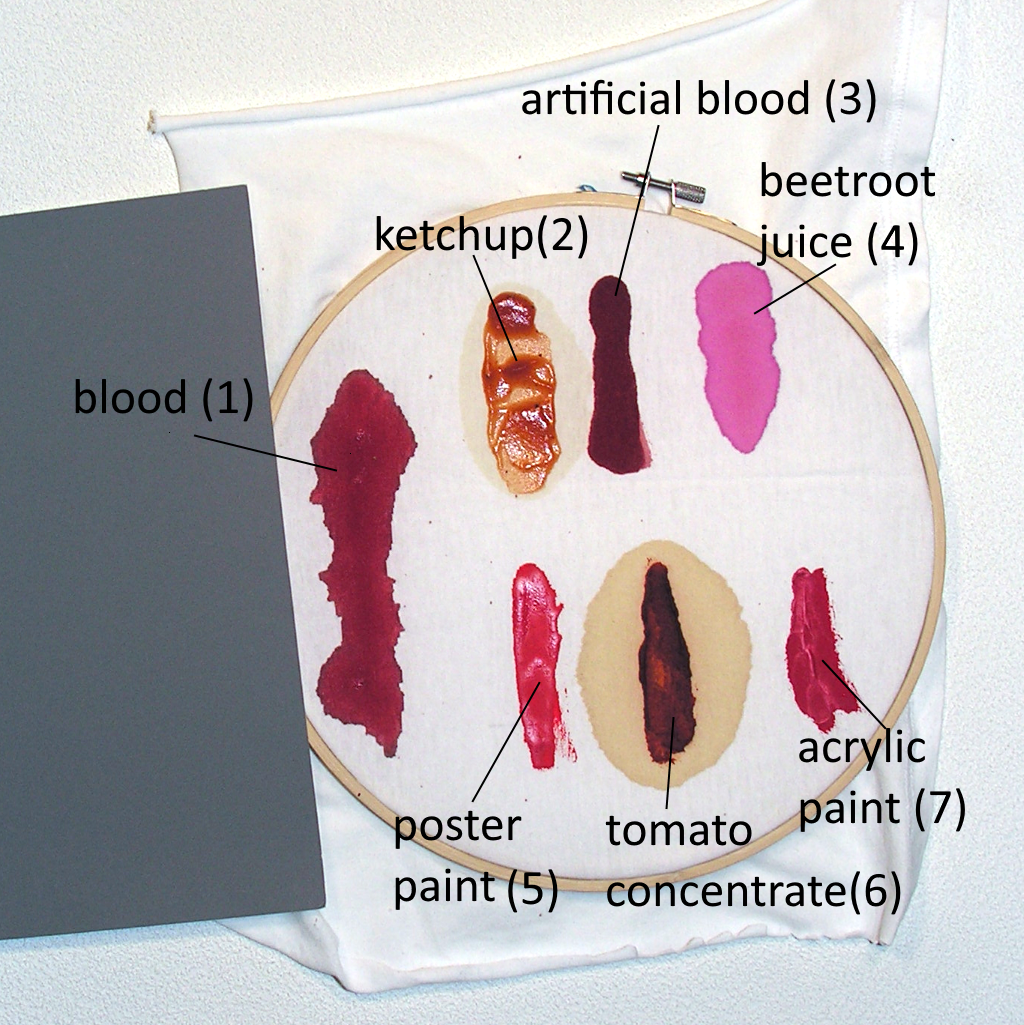
\includegraphics[width=0.44\textwidth]{figures/experiments_and_results/dataset_imgs/frame_image.png}
    \caption[Dataset classes overview.]{An image from the dataset documentation showing an overview of the classes present in the dataset \cite{Romaszewski2021}.}
    \label{fig:dataset_img}
    }
\end{figure}

\subsection{Classical Model Training and Evaluation}
Throughout this section, we will present training hyperparameters and resulting loss curves for each trained model containing LBAE and RBM models, which were trained with the CD-$1$ algorithm, simulated annealing, and quantum annealing. We will also present the evaluation metrics that we have obtained that justify proceeding further with the model, which we consider superior to other models. Obtained segmentation images and metrics computed for those images will be presented in the next section of this work.

At first, we will begin with training Latent Bernoulli Autoencoder (LBAE). As mentioned in Chapter \ref{methodology}, our approach relies on the work done in \cite{QBM4EO}. Since we changed only convolutional layers from two to one-dimensional, we will keep fixed hyperparameters of these layers as they were in \cite{QBM4EO}. Our experiments focused on studying the influence of changing batch size and learning rate.

The following values of batch size $b_i \in \{4, 8, 16\}$ and learning rate $\eta_i \in \{10^{-2}$, $10^{-3}$, $10^{-4}\}$ were chosen as a standard values \cite{raschka2019}. For each combination of these parameters, LBAE training was conducted, ultimately yielding nine trained models. Each model's performance was evaluated on a test dataset using Euclidean distance and spectral angle distance (SAD) metrics.

\noindent We will proceed with the LBAE model that obtained the lowest values of both metrics, that is the model trained with hyperparameters $b_i=4$ and $\eta_i=10^{-3}$.

Having trained the LBAE model, we determine a baseline for Restricted Boltzmann Machines (RBM) clusterization that we aim to surpass. For this purpose, we will use the $k$-means algorithm to perform clusterization on the test dataset for both scenarios, first for the data processed as described in Chapter \ref{methodology} and the data encoded by the LBAE encoder. To avoid the impact of how the centroids are initialized, we conducted the clustering ten times using different random seeds. The metrics introduced in the Section \ref{metrics_section} were computed for the resulting clustering. We will consider these metrics as baselines, visualized in the metrics plots computed for clustering using RBM.

We then proceeded with the RBM part and started with the CD-$1$ training procedure. Similar to the case of LBAE, we keep hyperparameters as they were in \cite{QBM4EO}, except for one of them --- a number of neurons in the hidden layer. We directed our efforts to explore the impact of the number of neurons in the RBM's hidden layer. RBM training experiments were conducted for the following number of neurons in hidden layer $h_i \in \{3, 4, \ldots, 28\}$, and those experiments were repeated ten times for different weights initialization.

Due to limited resources, we would like to proceed with further experiments involving simulated and quantum annealing using the best RBM model from those we obtained. However, it is unclear which of those models is better than others. To face the problem of choosing one model, we will use a V-measure, a meta-metric, whose value depends on homogeneity, completeness, and an additional $\beta$ parameter. Authors of \cite{Rosenberg2007} do not suggest how to choose $\beta$ value, however it is said that $\beta \in [0,1]$ promotes homogeneity. We will conduct an experiment, exploring how frequently, for which model we obtain the greatest value of V-measure for $\beta_i \in \{0, 0.01, \ldots, 1\}$. This experiment concluded that the RBM model with 23 neurons in the hidden layer was the most promising for the segmentation task. Figure \ref{fig:rbm_learning_cd} shows the learning curve for that model.

\begin{figure}[H]
    \centering
    {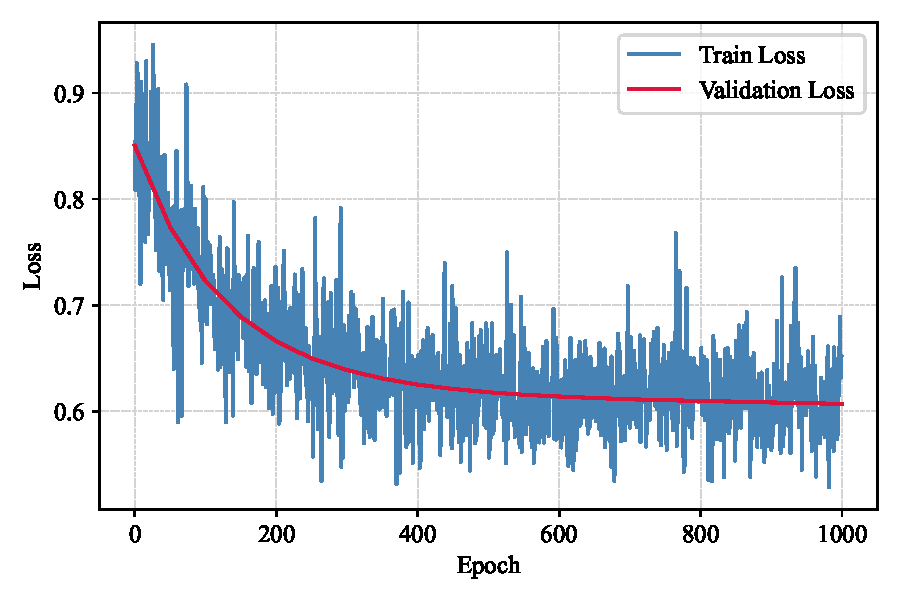
\includegraphics[width=0.85\linewidth]{figures/experiments_and_results/plot_loss/rbm_plot_loss_cd1.pdf}}
    \caption[Learning curve of the RBM from the CD-$1$ training.]{Learning curve of the RBM from the contrastive divergence (CD-$1$) training. The blue line represents the loss value on the training dataset, and the red line represents the loss value on the validation dataset.}
    \label{fig:rbm_learning_cd}
\end{figure}

After the RBM training, we faced the problem of RBM returning more unique labels than the target number of labels on ground-truth images. Following the idea that the RBM returned structure is hierarchical \cite{Decelle2023}, we could pass this structure to another algorithm, known as Agglomerative Hierarchical Clustering (AHC), and specify the target number of clusters.

For the segmentation images that we will create, we want to refer to a reliable baseline; for this task, we will again use the $k$-means algorithm. Figure \ref{fig:kmeans_segmentation} illustrates the clustering using $k$-means, and Figure \ref{fig:ground_truth_image} illustrates the ground truth image. Table \ref{tab:segmentation_metrics_comparison} shows metrics comparison for created segmentation images.

After obtaining baseline segmentation, we proceeded to create segmentation images using our network, which consists of an LBAE encoder, RBM, and AHC. These images are presented in Figure \ref{fig:cd1_rbm_ahc_complete_seg} and Figure \ref{fig:cd1_rbm_ahc_average_seg}.

\subsection{Quantum Model Training and Evaluation}
With the RBM hyperparameters determined, the next step of the project was to test the implemented training algorithm using a simulation annealer. For this task, we used D-Wave's implementation of a simulated annealing sampler \cite{DWaveDocumentation}. The training was repeated ten times for initialization with different weights, this time only for an RBM model containing 23 neurons in the hidden layer. We decided to save a model after every other hundred training epochs to execute an insightful analysis of model performance in the context of clusterization metrics.

Wanting to select the best model, we performed the procedure described in \ref{metrics_section} using the V-measure metric. This procedure concluded that the best one, from the obtained models, is the model saved on epoch 200. The learning curve of the RBM trained using the simulated annealer is shown in Figure \ref{fig:rbm_sa_learning_annealer}.

At this point, both RBM models have been trained with CD-$1$ and simulated annealing, so we proceed to train our model using quantum annealing. Again, we use the sampler provided by D-Wave \cite{DWaveDocumentation} and the automatic embedding of our problem into the target QPU Solver—Advantage 5.4. The training was repeated ten times for initialization with different weights, again only for an RBM model containing 23 neurons in the hidden layer. We decided to save a model after every other hundred training epochs.

As before, we repeat the procedure using the V-measure to obtain the model with the best performance in the context of evaluation metrics.  This procedure concluded that the best one, from the obtained models, is the model saved on epoch 300. The learning curve of the RBM trained using the quantum annealer is shown in Figure \ref{fig:rbm_qa_learning_annealer}.

\begin{figure}[H]
    \centering
    {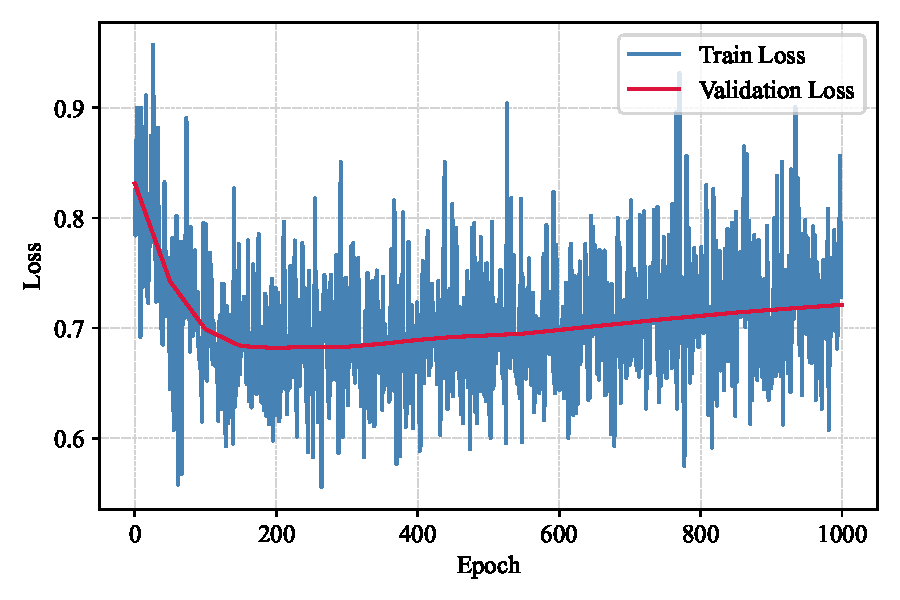
\includegraphics[width=0.85\textwidth]{figures/experiments_and_results/plot_loss/rbm_plot_loss_qa.pdf}
    \caption[Learning curve of the RBM from the QA training.]{Learning curve of the RBM from the quantum annealing training. The blue line represents the loss value on the training dataset, and the red line represents the loss value on the validation dataset.}
    \label{fig:rbm_qa_learning_annealer}
    }
\end{figure}

\subsection{Segmentation Results}
We will start showing our experiments results with our baseline segmentation obtained by using $k$-means algorithm on the Figure \ref{fig:kmeans_segmentation} and ground truth image on the Figure \ref{fig:ground_truth_image}. Next, we will present segmentations obtained by using our proposed model trained with contrastive divergence (CD-$1$) and followed by AHC using both linkage methods --- complete and average, those will be respectively Figure \ref{fig:cd1_rbm_ahc_complete_seg} and Figure \ref{fig:cd1_rbm_ahc_average_seg}. Similarly we will present segmentations for models trained with simulated annealing (SA) and quantum annealing (QA). For simulated annealing obtained images are Figure \ref{fig:sa_rbm_ahc_complete_seg} and Figure \ref{fig:sa_rbm_ahc_average_seg}, and for quantum annealing obtained images are Figure \ref{fig:qa_rbm_ahc_complete_seg} and Figure \ref{fig:qa_rbm_ahc_average_seg}.

\begin{figure}[h]
    \centering
    \begin{subfigure}{0.475\textwidth}
        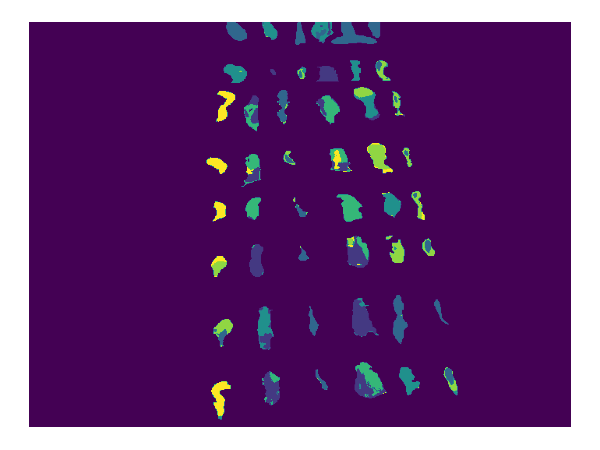
\includegraphics[width=\textwidth]{figures/experiments_and_results/kmeans_seg.pdf}
        \caption{$k$-means segmentation.}
        \label{fig:kmeans_segmentation}
    \end{subfigure}
    \hfill
    \begin{subfigure}{0.475\textwidth}
        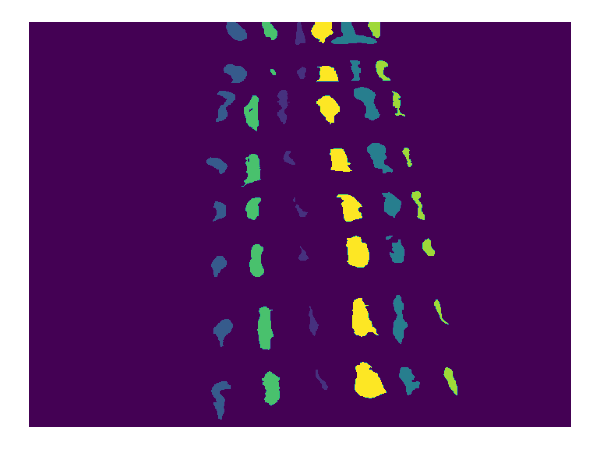
\includegraphics[width=\textwidth]{figures/experiments_and_results/gt.pdf}
        \caption{Ground truth.}
        \label{fig:ground_truth_image}
    \end{subfigure}

    \caption{Baseline segmentation by $k$-means and ground truth.}
    \label{fig:baseline_and_gt}
\end{figure}

\begin{figure}
    \centering

    \begin{subfigure}{0.475\textwidth}
        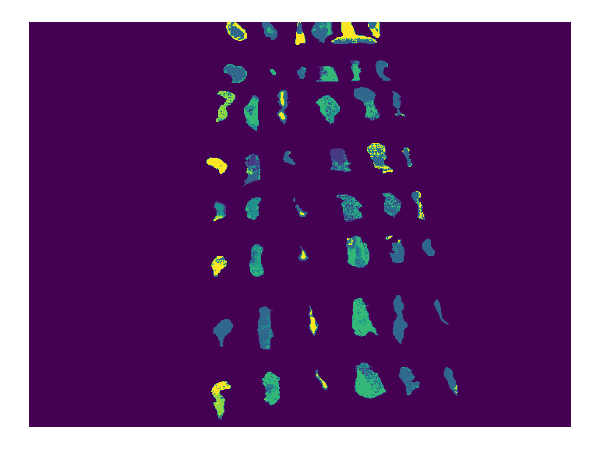
\includegraphics[width=\textwidth]{figures/experiments_and_results/segmentation/cd1/E_7_seg_nh=23_rs=70_link=complete.pdf}
        \caption{Segmentation by RBM trained by CD-$1$ with AHC using complete linkage.}
        \label{fig:cd1_rbm_ahc_complete_seg}
    \end{subfigure}
    \hfill
    \begin{subfigure}{0.475\textwidth}
        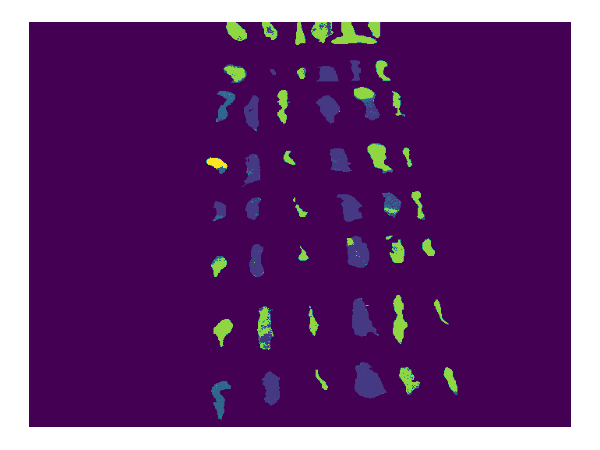
\includegraphics[width=\textwidth]{figures/experiments_and_results/segmentation/cd1/E_7_seg_nh=23_rs=70_link=average.pdf}
        \caption{Segmentation by RBM trained by CD-$1$ with AHC using average linkage.}
        \label{fig:cd1_rbm_ahc_average_seg}
    \end{subfigure}

    \begin{subfigure}{0.475\textwidth}
        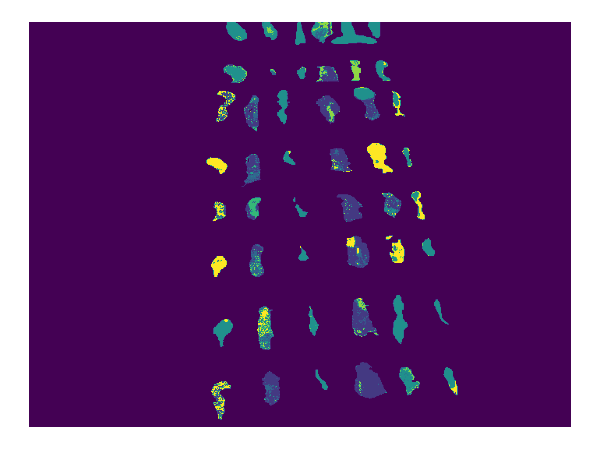
\includegraphics[width=\textwidth]{figures/experiments_and_results/segmentation/sa/rbm_nh=23_seed=50_epoch=200_ink=complete.pdf}
        \caption{Segmentation by RBM trained by SA with AHC using complete linkage.}
        \label{fig:sa_rbm_ahc_complete_seg}
    \end{subfigure}
    \hfill
    \begin{subfigure}{0.475\textwidth}
        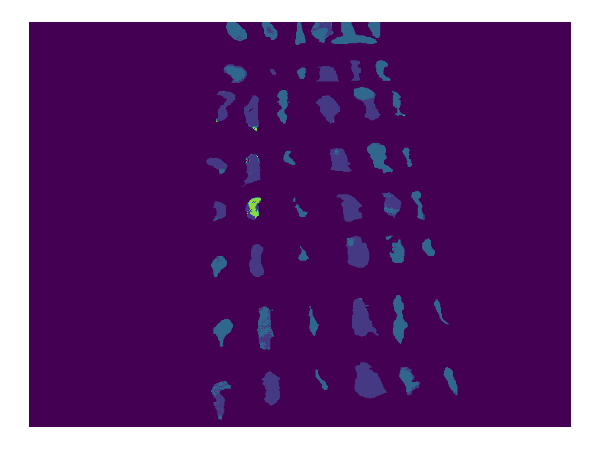
\includegraphics[width=\textwidth]{figures/experiments_and_results/segmentation/sa/rbm_nh=23_seed=50_epoch=200_ink=average.pdf}
        \caption{Segmentation by RBM trained by SA with AHC using complete linkage.}
        \label{fig:sa_rbm_ahc_average_seg}
    \end{subfigure}

    \begin{subfigure}{0.475\textwidth}
        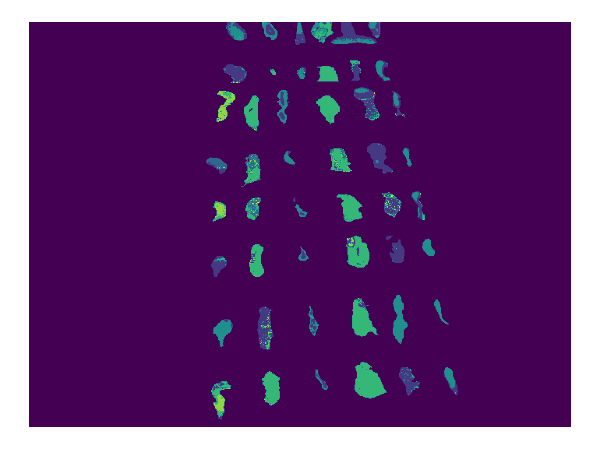
\includegraphics[width=\textwidth]{figures/experiments_and_results/segmentation/qa/rbm_nh=23_seed=10_epoch=300_link=complete.pdf}
        \caption{Segmentation by RBM trained by QA with AHC using complete linkage.}
        \label{fig:qa_rbm_ahc_complete_seg}
    \end{subfigure}
    \hfill
    \begin{subfigure}{0.475\textwidth}
        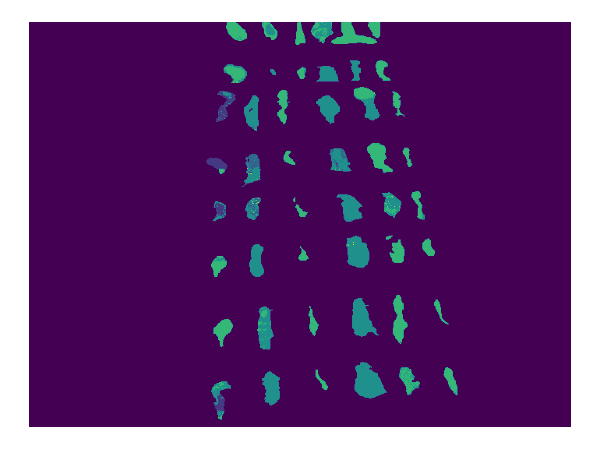
\includegraphics[width=\textwidth]{figures/experiments_and_results/segmentation/qa/rbm_nh=23_seed=10_epoch=300_link=average.pdf}
        \caption{Segmentation by RBM trained by QA with AHC using complete linkage.}
        \label{fig:qa_rbm_ahc_average_seg}
    \end{subfigure}
    
    \caption{Comparison of the obtained segmentations.}
    \label{fig:comparison_seg}
\end{figure}

\noindent A summary of the computed evaluation metrics such as homogeneity, completeness, adjusted rand score (ARS) and rand score (RS) for each segmentation obtained is presented collectively in Table \ref{tab:segmentation_metrics_comparison}.

\begin{table}
    \centering
    \caption[Comparison of clustering evaluation metrics for baseline segmentation and segmentation produced by our models.]{Comparison of clustering evaluation metrics for baseline segmentation and segmentation produced by our models. Here, RBM+AHC-C denotes the RBM with AHC using complete linkage, and RBM+AHC-C denotes the RBM with AHC using average linkage.}
    \begin{tabular}{@{} llcccc @{}}
        \toprule
        \textbf{Metric} & \textbf{Training} & \textbf{$k$-means} & \textbf{RBM} & \textbf{RBM+AHC-C} & \textbf{RBM+AHC-A} \\
        \midrule
        \textbf{Homogeneity} & -- & 0.368 & -- & -- & -- \\
                             & CD-$1$ & -- & 0.492 & 0.232 & 0.243 \\
                             & SA  & -- & \textbf{0.510} & 0.231 & 0.171 \\
                             & QA  & -- & 0.505 & 0.254 & 0.260 \\
        \midrule
        \textbf{Completeness} & -- & 0.354 & -- & -- & -- \\
                              & CD-$1$ & -- & 0.239 & 0.257 & 0.416 \\
                              & SA  & -- & 0.244 & 0.266 & 0.381 \\
                              & QA  & -- & 0.282 & 0.319 & \textbf{0.445} \\
        \midrule
        \textbf{ARS} & -- & 0.244 & -- & -- & -- \\
                     & CD-$1$ & -- & 0.163 & 0.129 & 0.242 \\
                     & SA  & -- & 0.180 & 0.199 & 0.181 \\
                     & QA  & -- & \textbf{0.308} & 0.284 & 0.246 \\
        \midrule
        \textbf{Rand Score} & -- & 0.769 & -- & -- & -- \\
                            & CD-$1$ & -- & 0.793 & 0.690 & 0.660 \\
                            & SA  & -- & \textbf{0.799} & 0.711 & 0.590 \\
                            & QA  & -- & 0.790 & 0.729 & 0.656 \\
        \bottomrule
    \end{tabular}
    \label{tab:segmentation_metrics_comparison}
\end{table}

\subsection{Conclusions}
Analyzing obtained metrics on the segmentation images, we notice that almost all metrics improve their value for RBM trained with QA, and if they are not improved, they are close to the best-obtained value. For a model that does not use AHC, we note the consistent improvement of the metrics while changing the RBM training algorithm from CD-1 through SA to QA. For the metrics homogeneity and ARS, the RBM model trained with QA surpassed the baseline value, which was set by the $k$-means algorithm. The use of the AHC algorithm in combination with RBM affects clustering characteristics. First, AHC improves the completeness metric, especially when using the RBM version trained with Quantum Annealing. At the same time, adding AHC reduces the clusters' homogeneity. 

\section{Summary}\label{summary}
This work proposes a hybrid neural network architecture --- Latent Bernoulli Autoencoder's encoder connected with Restricted Boltzmann Machines for multispectral image segmentation. Firstly, the LBAE's encoder part is utilized for dimensionality reduction and encoding spectral data to a binary representation, which is necessary for RBM. Secondly, we use RBM to perform clustering on the encoded spectral pixels.

The proposed architecture and experiments confirmed the effectiveness of applying quantum annealing techniques and RBM models for the segmentation of multispectral images since we achieved better segmentations, in terms of observed metrics than the baseline segmentation obtained using standard algorithm --- $k$-means. The results suggest the potential for further research on using quantum annealing in the image processing field.

\addcontentsline{toc}{section}{Bibliography}
\printbibliography

\end{document}